\documentclass[ignorenonframetext]{beamer}
%\documentclass[11pt]{article}
%\usepackage{beamerarticle}
\mode<article>{\usepackage{fullpage}
  \usepackage{palatino}
  \usepackage{mathpazo}
  \usepackage{graphicx}
}

\mode<presentation>{\usetheme{Boadilla}}

\usepackage[latin1]{inputenc}
\usepackage{amsmath}

\title[Radiation kriging]{Spatial kriging of radiation data}
\subtitle{(Statistics for national security)}
\author{Alex Reinhart}
\institute{Applied Research Labs}
\date{May 1, 2013}

\begin{document}

\maketitle

\begin{frame}
\titlepage
\end{frame}

Imagine collecting this data (well, a noisy version) at every point in space.

\begin{frame}
  \begin{figure}
    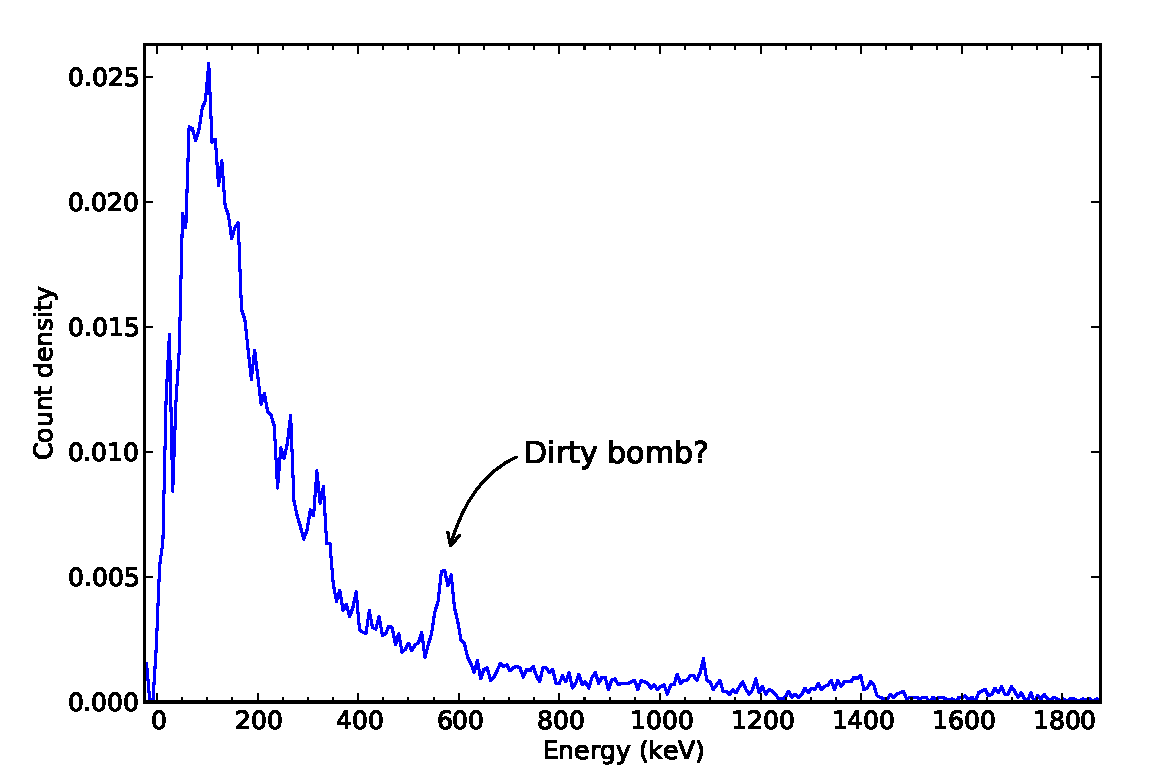
\includegraphics[width=110mm]{figures/talk-bomb-spectrum.pdf}
    \caption{Gamma ray spectrum collected at Pickle Research Campus.}
  \end{figure}
\end{frame}

We would like to be able to collect this data one day, then return the next day
and tell if it is substantially different from the day before. This is better
than simply looking for more radioactive areas, because:

\begin{frame}
  \begin{figure}
    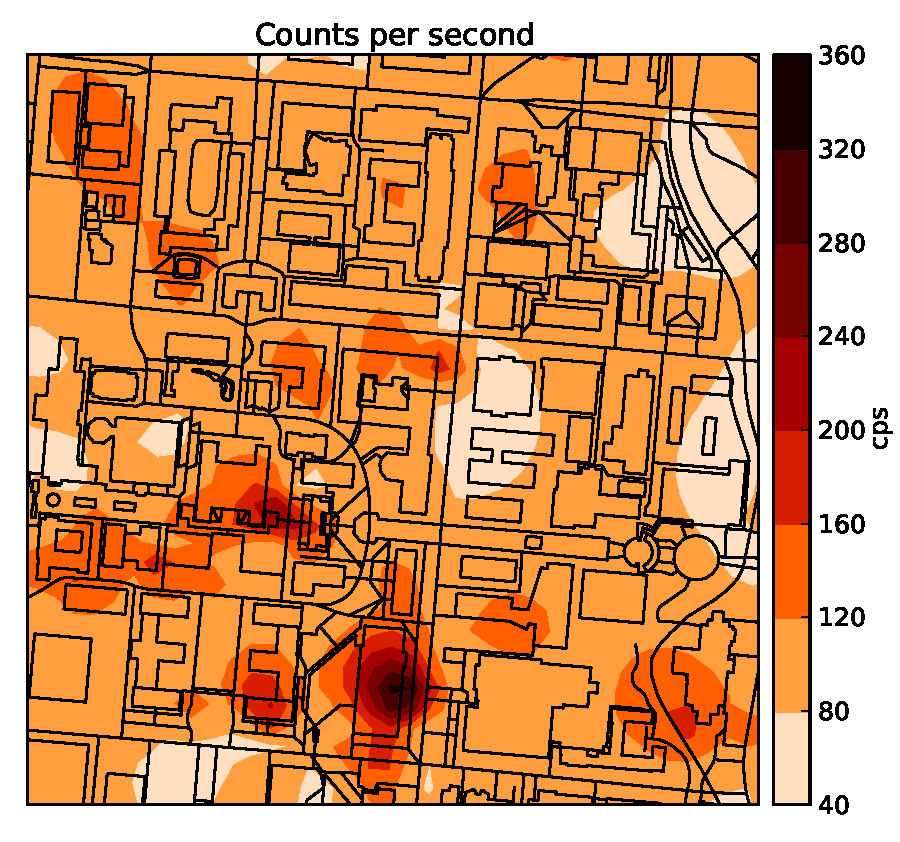
\includegraphics[width=85mm]{figures/talk-campus-map.pdf}
    \caption{The University of Texas campus radiation map.}
  \end{figure}
\end{frame}

\begin{frame}{Kriging model}
  The model:
  \begin{align}
    Z(\mathbf{s}) | Y(\mathbf{s}) &\sim \text{Poisson}(t(\mathbf{s})
    Y(\mathbf{s}))\\
    C_Y(\mathbf{s}, \mathbf{s'}) &= \sigma_Y^2 - \gamma_Y (\mathbf{s},
    \mathbf{s'})
  \end{align}

  We assume we can predict count rates with
  \begin{equation}
    \hat{Y}(\mathbf{s}_0) = \sum_{\alpha=1}^n \lambda_\alpha
    \frac{Z(\mathbf{s}_\alpha)}{t(\mathbf{s}_\alpha)}.
  \end{equation}
\end{frame}

\begin{frame}{Kriging system}
  \begin{align}
    \sum_{\beta=1}^n \lambda_\beta C(\mathbf{s}_\alpha, \mathbf{s}_\beta) +
    \lambda_\alpha \frac{m}{t(\mathbf{s}_\alpha)} + \mu &= C(\mathbf{s}_\alpha,
    \mathbf{s}_0)\qquad \text{for } \alpha = 1, \ldots, n\\
    \sum_{\alpha=1}^n \lambda_\alpha &= 1
  \end{align}
  where \(m\) is the mean of \(Y\) and \(\mu\) is a Lagrange multiplier.
\end{frame}

\begin{frame}{Anomaly detection}
  \begin{itemize}
    \item Estimate the variogram using a model:
      \begin{equation}
        \gamma_Y(h) = c\left(1 - \exp \left(- \left(\frac{h}{a}\right)^d \right)\right)
      \end{equation}
    \item Collect background data and use it to make a set of predictions
    \item Compare new data (aggregated into small spatial bins) to old predictions
  \end{itemize}
\end{frame}

\begin{frame}{Anomaly detection}
  \begin{align}
    Z(\mathbf{s}) | \hat Y(\mathbf{s}) t(\mathbf{s}) &\sim \text{Poisson}(\hat Y(\mathbf{s})
    t(\mathbf{s}))\\
    \hat Y(\mathbf{s}) t(\mathbf{s}) &\sim \text{Gamma}(a, (1-b)/b)\\
    a &= \frac{\hat Y^2}{\sigma_{\hat Y}^2}\\
    b &= \frac{t(\mathbf{s}) \sigma_{\hat Y}^2}{\hat Y + t(\mathbf{s}) \sigma_{\hat Y}^2}
  \end{align}

  Hence we can integrate (giving us a negative binomial) and determine \(P(Z)\)
  to compare new data against.
\end{frame}

\end{document}